\section{Traversing Potential Energy Surfaces}
\label{sec:pes}

This section introduces the idea of potential energy surfaces (PESes) and discusses their creation and exploration.

%This secion shortly introduces a few concepts that are important to the work being presented.

\bit
\item Forces as inverse gradient. (Hellmann-Feynman?)
%\item Maybe this section can be called "Potential Energy Surfaces" or something like that.
\eit

\incomplete

\section{The Schr\"odinger Equation}
\label{sec:schrodinger}

A central theme in atomic simulations is the solution of the Schr\"odinger equation~\cite{schrodinger-equation-1926}, which is the quantum analogue of Newton's equations of motion~\cite{newton-latin}, governing the motion of the electrons and nuclei, as well as any other observables.
For a non-relativistic system of $N = N_e + N_n$ particles ($N_e$ electrons and $N_n$ nuclei), the time independant Schr\"odinger equation \tred{(Why not the time dependant one?)},
\beq{schrodinger-basic}
 \widehat{H}\Psi = E\Psi,
\eeq
must be solved in order to calculate the total energy of the system, $E$, and the wave function, $\Psi \equiv \Psi(\vr_1, \vr_2, \ldots, \vr_{N_e}, \vR_1, \vR_2, \ldots, \vR_{N_n})$, which depends on the spatial coordinates, $\vr_i$, of each electron and, $\vR_i$, each nuclei, using the total energy operator (more commonly referred to as the Hamiltonian),
\beq{hamiltonian}
\widehat{H} = \sum_i^{N}\widehat{T}_i  + \widehat{V}.
\eeq
Similar to classical systems the Hamiltonian encompasses both kinetic, $\widehat{T}_i = -\nabla_i^2/2$, \footnote{In atomic units} and potential, $\widehat{V} = V(\vR, \vr)$, effects, represented in the traditional R-basis, which will be used exclusively in this thesis.
Though it may look innocent, solving the Schr\"odinger equation, which is a second order partial derivative problem, is a daunting task and in most cases significant approximations must be made.
Efforts to solve the Schr\"odinger equation are discussed below in \fref{sec:methods-qm}.

% ------------------------------------------------------------------
\section{The Born-Oppenheimer Approximation}
\label{sec:born-oppenheimer}

In order to simplify --- and in many cases, make possible --- quantum calculations of large atomic systems, the difference in weight of the electrons and the nuclei\footnote{\mytilde 4 orders of magnitude for hydrogen and more for the heavier elements.} is exploited by performing the calculations in two steps.
First, while the nuclei are kept motionless by excluding their kinetic operator from the Hamiltonian (\fref{eq:hamiltonian}), the electronic wavefunction and energy are determined followed by a calculation for the motion of the nuclei.
The assumption is, essentially, that for any motion of the nuclei, the electrons will move instantly, and remain in their ground state, to accommodate and is commonly known as the Born-Oppenheimer approximation\cite{born-oppenheimer-1927}.

\figmiss{Example PES}

This decoupling allows for a mapping of the potential energy as a function of the nuclear coordinates (commonly referred to as the potential energy surface or PES), as opposed to the continuum of PESes which exist should the motion of the nuclei and electrons be determined simultaneously.
PESes are, generally, not known \textit{a priori} and much effort is spent on traversing them to discover interesting features, such as minima, which represent stable structures, or, as we shall see below, reaction pathways.

For many systems this is a good approximation and has even proved useful for metallic systems --- for which its use could be considered questionable due to the lack of a band gap --- \expand Need to think a bit more about this...

\bit
\item Excited electronic states
\item Good when the gap between electronic states is larger than the energyscale of the nuclear motion.
\item Should be bad for metallic systems but has proved useful nevertheless. \footnote{see \url{http://www.nature.com/nmat/journal/v6/n3/pdf/nmat1846.pdf}}
\eit

All the work carried out in this thesis employs the Born-Oppenheimer approximation.

% ------------------------------------------------------------------
%\subsection{Eigenmodes / Eigenvalues}
%\label{sec:eigenmodes}
%
%\placeholder

% ------------------------------------------------------------------
%\subsection{Reduced Vector-space}
%\label{sec:reduced-space}
%
%\placeholder

% ------------------------------------------------------------------
\subsection{The Hessian Matrix}
\label{sec:hessian}

For a real function $f$ of $n$ variables, $\vect{x} = (x_1, x_2, \ldots, x_n)$,
there exists an $n\times n$ matrix, $H$, which contains all the second partial derivatives, if they exist,
\beq{hessian-matrix}
H =
\begin{bmatrix}
\vspace{0.5em} % To create a bit of space AFTER the first line.
\frac{\partial^2f}{\partial x_1^2} &
\frac{\partial^2f}{\partial x_1 \partial x_2} &
\cdots &
\frac{\partial^2f}{\partial x_1 \partial x_n} \\

\frac{\partial^2f}{\partial x_2 \partial x_1} &
\frac{\partial^2f}{\partial x_2^2} & 
\cdots &
\frac{\partial^2f}{\partial x_2 \partial x_n} \\

\vdots & \vdots & \ddots & \vdots \\

\frac{\partial^2f}{\partial x_n \partial x_1} &
\frac{\partial^2f}{\partial x_n \partial x_2} &
\cdots &
\frac{\partial^2f}{\partial x_n^2} &
\end{bmatrix}.
\eeq
The second derivative of a function represents, in particular, information about its local curvature, or how rapidly the first derivative changes.

$H$ is named after the German mathematician Ludwig Otto Hesse and is commonly referred to as the Hessian matrix, or Hessian for short.~\citemiss{}

In the context of atomic simulations $n$ is generally 3 times the number of atoms in the system, as each one has 3 independant degrees of freedom.
The function in question is often the potential energy of the system, whose negative gradient is commonly referred to as the force.
In most modern software packages both the potential energy and force are readily available while the second derivatives are, generally, not available without explicit and, often, costly calculations.

\section{Steepest Descent Paths}
\label{sec:sdps}

\figmiss{Showing a few general SDPs and at least one MEP and one ridge}

Steepest Descent Paths (SDPs) are paths on a multidimensional function, $f$, for which there is no perpendicular gradient component,
\beq{sdp-definition}
\nabla f - (\nabla f \cdot \tau)\tau = \vect{0}, \tblue{ATH: vectors?}
\eeq
where $\tau$ is the tangent to the path.
They can be created by following the negative gradient until it vanishes.
SDPs can begin anywhere, apart from points with a vanishing gradient, but, generally, end at minima (most common) or \sap{}s.
Two sorts of SDPs are of particular interest for the work presented in this thesis, both of which are discussed below.

\bit
\item Missing citation, maybe it is okay to use \cite{gradient-extremals-ruedenberg-1993}
\eit

\subsection{Minimum Energy Paths}
\label{sec:meps}

\bit
\item Need a good definition and/or citation.
%Check this reference:
%Transition-Path Theory and Path-Finding Algorithms for the Study of Rare Events
%(Weinan E and Eric Vanden-Eijnden)
\eit

The Minimum Energy Path (MEP) is specific SDP, used in the context of theoretical reaction chemistry and represents a likely reaction path on the PES.
The MEP's formal definition is generally the same as for any SDP (\fref{eq:sdp-definition}) but with the added criteria that the energy must be at a minimum perpendicular to the path~\cite{neb-polemic-henkelman1},
\beq{mep-definition}
\text{\expand}
\eeq

\subsection{Ridges}
\label{sec:ridges}

Similar to MEPs, ridges are specific SDPs, except with beginning and end points in \sap{2}s and \sap{1}s respectively.
Of course, MEPs do not exists near \sap{2}s, and the anlogue ends there as the criteria for ridges \expand

\bit
\item Need a good definition and/or citation.
\eit


\subsection{Saddle Points \tblue{[LOCATION PENDING]}}
\label{sec:sps}

\bit
\item Positioning this bit is rather difficult. Should it be in the "random stuff" section, the HTST section or the saddle-point methods section?
\item \figmiss{I'd like to have a saddle for horse riding as a comparison here.}
\eit

Saddle points are stationary points, i.e. with zero gradient, on a multidimensional function, $f(\vR)$, that are neither maxima nor minima.

\begin{figure}[h]
  \begin{center}
  \subfigure[2D saddle point][2D saddle point, $f(x=0, y=0) = x^2 - y^2$. A minimum is the $x$ direction and a maximum in the $y$ direction]{
    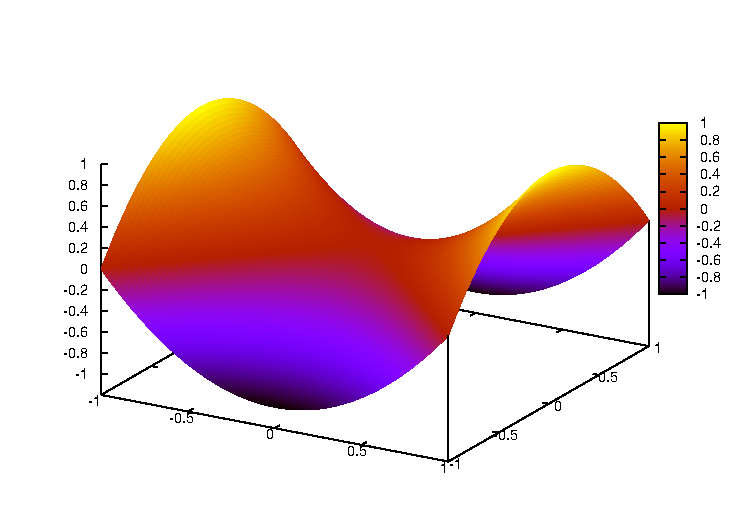
\includegraphics[width=0.6\linewidth]{saddle-point}
    \label{fig:2d-saddle-point}
    }
  \subfigure[1D saddle point][1D saddle point, $f(x=0) = x^3$. Neither a maximum nor a minimum but the gradient is vanishing.]{
    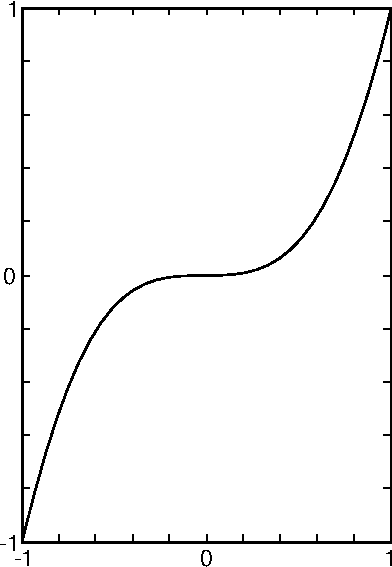
\includegraphics[width=0.26\linewidth]{saddle-point-1d}
    \label{fig:1d-saddle-point}
    }
    \parbox{0.85\linewidth}{
      \caption{Examples of first order saddle points.
      }
      \label{fig:saddle-points}
    }
  \end{center}
\end{figure}

A common view of a saddle (point) can be found in \fref{fig:2d-saddle-point}, as the function $f(x, y) = x^2 - y^2$ which near $(x,y) = (0,0)$ resembles a saddle, used when riding horses, curving upwards (along the horse) in one direction and downwards in the other (parallel to the horse).
This image of a saddle point lacks a few elements to be to tell their whole story but acts as a good general case.
On functions of higher dimensionality than $2$, different orders of saddle points are possible.
The order of the saddle point is decided by the amount of directions that are not at a minimum, or the non-positive eigenvalues of the Hessian.
As such, \fref{fig:2d-saddle-point} shows a first order saddle point on a two dimensional function.
In this thesis, saddle points of order $N$ will be indicated by \sap{N} from here on.

The Hessian at the \sap{} displayed in \fref{fig:2d-saddle-point} has one negative eigenvalue, however, a saddle point with one or more vanishing eigenvalues is also possible, such as the 1D example $f(x = 0) = x^3$, seen in \fref{fig:1d-saddle-point}.

Locating \sap{}s in multiple dimensions is a non-trivial task as only a limited number of steepest decent paths lead to each one while the majority lead to minima.
A number of schemes  for locating \sap{1}s have been suggested (see \cite{sp-mep-review-2002} for a reivew), out of which two popular ones are discussed below, in \fref{sec:saddle-point-methods}: The Dimer method and the Nudged Elastic Band method.
Furthermore, an extension to these methods for finding higher order \sap{}s is presented in \fref{chap:erm}.

In the context of atomic simulations, \sap{}s are important in describing reactions and reaction rates.

\subsection{Optimisers}
\label{sec:optimisers}

\bit
\item Introduce optimisers (minimisers, is there a difference)
\item What are they used for?
\item Possibly introduce specific algorithms: Steepest Descent, FIRE, (L)BFGS
\eit

\placeholder

% ------------------------------------------------------------------
